\chapter{Detalles de la implementación}

\section{Definición de las interfaces responsive} \label{sec:def_interfaces_responsive}

Una interfaz responsive es un tipo de interfaz que se adapta al dispositivo donde se esté visualizando el sitio web. Para conseguir esta adaptación se hace uso de una cierta estructura del lenguaje CSS. Esta estructura son los @media \footnote{\url{https://www.w3schools.com/cssref/css3_pr_mediaquery.asp}}. Dentro de esta estructura se puede indicar que restricciones queremos que se cumplan sobre la pantalla, como pueden ser el máximo y el mínimo, tanto de ancho como de alto de la pantalla. Con estas restricciones se van generando los estilos propios de cada dispositivo.

Las restricciones que se han utilizado son las mostradas en la Tabla \ref{tab:restri_tam_dispo}.

\begin{table}[h]
\centering
\resizebox{\textwidth}{!}{%
\begin{tabular}{c|cc|cc|}
\cline{2-5}
\multicolumn{1}{l|}{} &
  \multicolumn{2}{c|}{\cellcolor[HTML]{FFFC9E}\textbf{Altura}} &
  \multicolumn{2}{c|}{\cellcolor[HTML]{FFFC9E}\textbf{Anchura}} \\ \cline{2-5} 
\multicolumn{1}{l|}{} &
  \multicolumn{1}{c|}{\cellcolor[HTML]{FFCE93}\textbf{Max.}} &
  \cellcolor[HTML]{FFCE93}\textbf{Min.} &
  \multicolumn{1}{c|}{\cellcolor[HTML]{FFCE93}\textbf{Max.}} &
  \cellcolor[HTML]{FFCE93}\textbf{Min.} \\ \hline
\multicolumn{1}{|c|}{\cellcolor[HTML]{FFFC9E}\textbf{Portátil}} &
  \multicolumn{1}{c|}{1080px} &
  751px &
  \multicolumn{1}{c|}{1920px} &
  1025px \\ \hline
\multicolumn{1}{|c|}{\cellcolor[HTML]{FFFC9E}\textbf{Tablet Horizontal}} &
  \multicolumn{1}{c|}{750px} &
  500px &
  \multicolumn{1}{c|}{1024px} &
  751px \\ \hline
\multicolumn{1}{|c|}{\cellcolor[HTML]{FFFC9E}\textbf{Tablet Vertical}} &
  \multicolumn{1}{c|}{1024px} &
  751px &
  \multicolumn{1}{c|}{750px} &
  500px \\ \hline
\multicolumn{1}{|c|}{\cellcolor[HTML]{FFFC9E}\textbf{Móvil}} &
  \multicolumn{1}{c|}{850px} &
  500px &
  \multicolumn{1}{c|}{400px} &
  200px \\ \hline
\end{tabular}%
}
\caption{Restricciones de tamaño de pantalla para los dispositivos}
\label{tab:restri_tam_dispo}
\end{table}

Para obtener estas medidas de pantalla se han analizado varios dispositivos de cada uno de los tipos de dispositivo utilizados en la Tabla \ref{tab:restri_tam_dispo}.

Un caso de uso de distintos estilos según el dispositivo, es la visualización de la descripción de la página principal y del \gls{mockup}. Cuando el dispositivo tiene la suficiente anchura, se muestran ambos elementos en paralelo, como se puede ver en la Figura \ref{fig:responsive_portatil} (Portátil, Tablet Horizontal); mientras que cuando la anchura no lo permite, se muestran uno detrás del otro como se puede ver en la Figura \ref{fig:responsive_tablet} (Tablet Vertical, Móvil).

\begin{figure}[h]
\centering
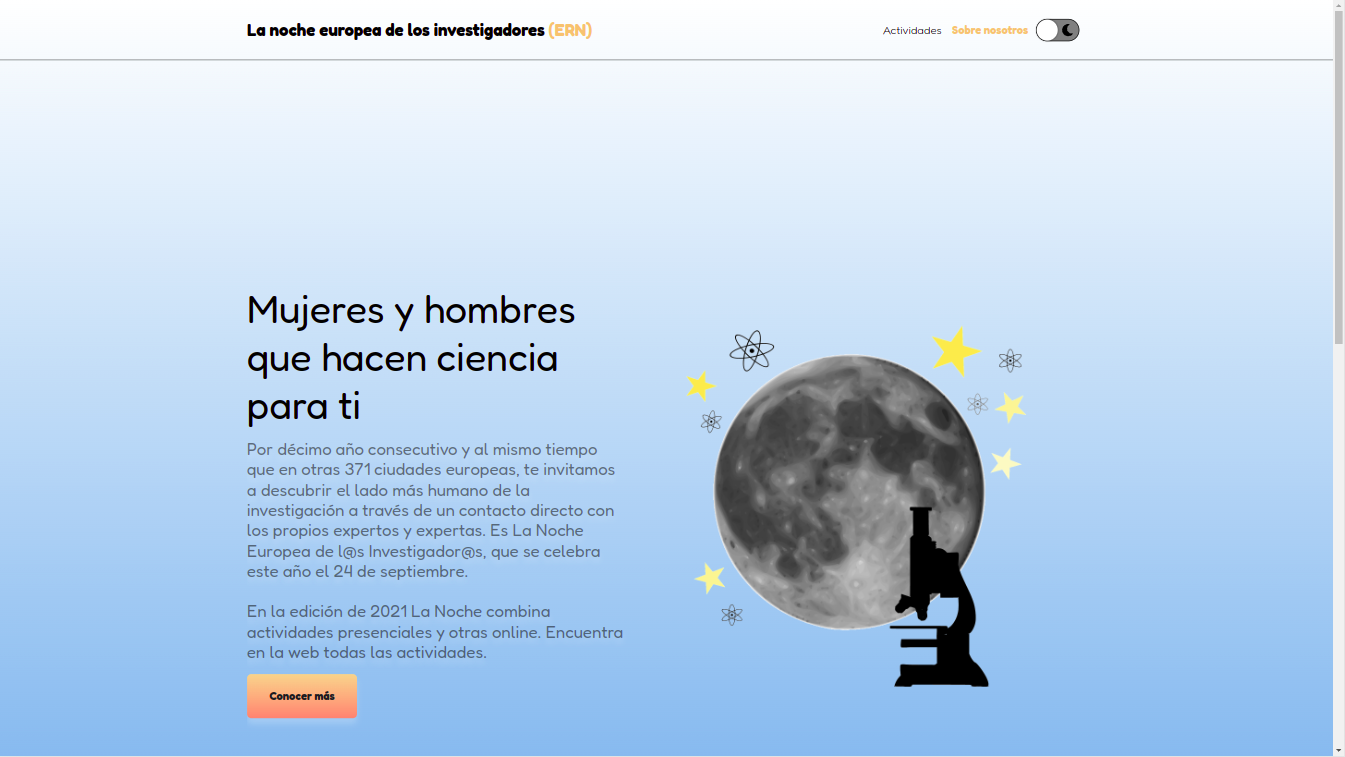
\includegraphics[width=0.8\textwidth]{imagenes/07_Implementacion/responsive_portatil.png}
\caption{Interfaz responsive usando el portátil}
\label{fig:responsive_portatil}
\end{figure}

\begin{figure}[h]
\centering
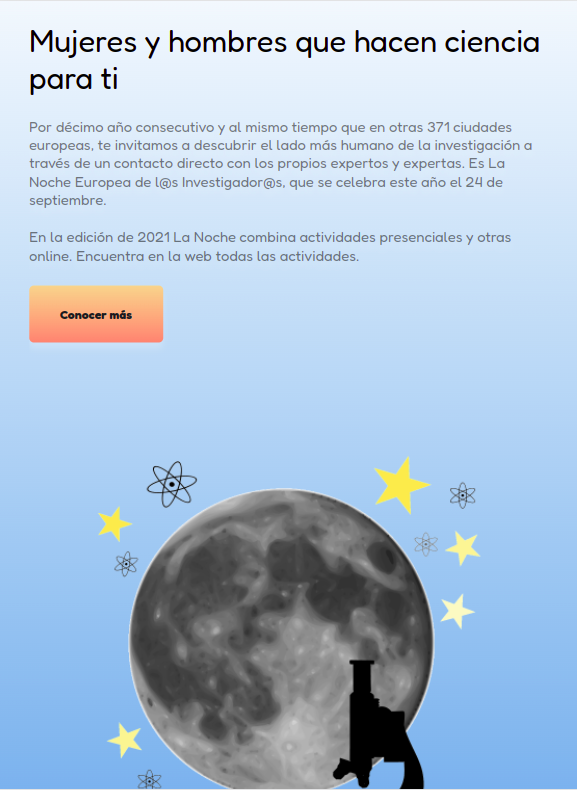
\includegraphics[width=0.6\textwidth]{imagenes/07_Implementacion/responsive_tablet.png}
\caption{Interfaz responsive usando la tablet en orientación vertical}
\label{fig:responsive_tablet}
\end{figure}

Esta filosofía de creación de sitios web permite crear varios sitios web definiendo una única vez los elementos que forman el sitio web y definiendo varios estilos que modifiquen los atributos de esos elementos.


\section{Funcionamiento del interruptor de cambio de tema} \label{sec:funcio_interruptor}

Suponiendo que hemos definido ambos temas, para generar el interruptor será necesario crear un elemento nuevo en la barra de navegación de las distintas secciones del sitio web. El interruptor será un elemento compuesto por dos espacios, donde en cada espacio habrá un icono de un sol y una luna respectivamente; y una bola que se encuentra en el interior de estos dos espacios y que se desplaza del extremo izquierdo al extremo derecho y viceversa.

Una vez definidos los componentes de este interruptor es hora de explicar como se ha implementado el movimiento del interruptor para cambiar de tema. Este movimiento se simula a través del cambio del estilo del interruptor. En un principio el interruptor tiene el estilo \textit{switch\_dark\_mode}, el cual coloca la bola de su interior en el extremo izquierdo, dejando ver el icono de la luna. De esta forma estamos indicando que al hacer clic en el interruptor se pasará al modo oscuro que está asociado con el icono de la luna. Dentro del estilo \textit{switch\_dark\_mode} se definen todos los atributos del espacio que ocupa el interruptor, ya que los atributos de la bola se definen en la parte \textit{::after} del estilo \textit{switch\_dark\_mode}. Los atributos de la bola se definen en esta sección porque se trata de un pseudo-elemento del interruptor. Hasta ahora tendremos los estilos del interruptor cuando está inactivo y, por lo tanto, el sitio web se encuentra en el tema claro. Falta definir los atributos que cambiaran del estilo del interruptor al activar el interruptor. Para tener de base los atributos del interruptor en modo inactivo y solamente tener que modificar el color y la posición de la bola al activar el interruptor, se añadirá o eliminará el estilo \textit{active} al estilo \textit{switch\_dark\_mode}. En este nuevo estilo \textit{active} se indica cuál será el color del interruptor cuando se encuentra activo y sitúa la bola en el extremo derecho del interruptor, dejando ver el icono del sol, el cual está asociado con el modo claro y, por lo tanto, indicando que si se vuelve a pulsar sobre el interruptor se desactivará el interruptor y se volverá al modo claro.

Visualmente, el estado del interruptor se muestra distinto en modo inactivo (
\includegraphics[width=0.07\textwidth]{imagenes/07_Implementacion/switch_inactive.png}) que en modo activo (
\includegraphics[width=0.07\textwidth]{imagenes/07_Implementacion/switch_active.png}).

Por último, falta implementar la parte dinámica de este interruptor, ya que hasta ahora únicamente hemos definido los elementos y los estilos que forman el interruptor, pero es necesario que el cambio de estilos del interruptor se realice mientras se utiliza el sitio web. Para implementar esta funcionalidad se crea un script de Javascript, el cual es incluido en todas las secciones del sitio web para poder hacer uso del interruptor en cada una de ellas. Dentro de este script se obtiene el elemento HTML que contiene al interruptor y posteriormente se define un evento de clic al pulsar sobre el interruptor. Al definir este evento, asignamos la ejecución de una función al hacer clic sobre el interruptor. La función a ejecutar consiste en dos comandos toggle. Lo que hace un comando toggle en Javascript es añadir el estilo que se le indica, al elemento sobre el que se ejecuta el comando; o eliminar el estilo si el elemento sobre el que se ejecuta el comando ya contiene el estilo. En primer lugar, se añade o elimina el estilo \textit{dark\_mode} a todos los elementos de la página web. Y en segundo punto, se añade o elimina el estilo \textit{active} al interruptor.

\section{Implementación del despliegue del menú lateral} \label{sec:despli_menu_lateral}

Para la implementación de esta funcionalidad serán necesarios dos elementos. Por un lado, el botón para desplegar el menú; y, por otro lado, el propio menú lateral.

El botón para desplegar el menú consiste en un simple botón de HTML, al cual se le añade un icono (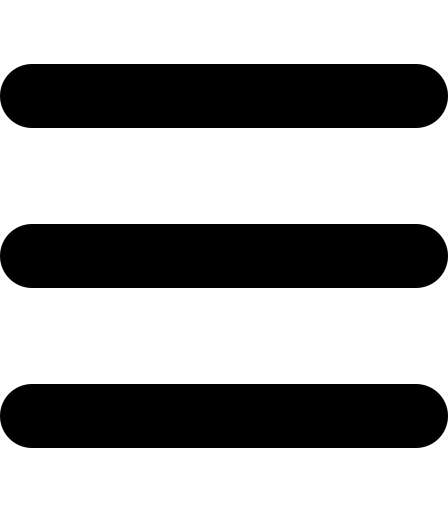
\includegraphics[width=0.03\textwidth]{imagenes/07_Implementacion/bars-solid.png}).

Para implementar el despliegue y la ocultación del menú lateral se hace uso de la misma táctica que con el interruptor (Apartado \ref{sec:funcio_interruptor}) para el cambio de tema de colores. Esta táctica consiste en utilizar distintos estilos para variar la apariencia de los elementos que deseamos. Siguiendo esta táctica se creará el estilo \textit{sidebar}, que afecta al menú lateral. Este primer estilo mantiene oculto al menú lateral. En segundo lugar, se genera el estilo \textit{deploy}, que también afecta al menú lateral, y el cual hace visible al menú lateral. Con estos dos estilos podemos implementar la funcionalidad del menú lateral.

Para implementar la funcionalidad se hace empleo de un script de Javascript, el cual se coloca en todas las secciones del sitio web, al igual que se hace con el script para el interruptor. Dentro de este script se obtiene tanto el botón de despliegue como el elemento que contiene al menú lateral. Por último, asignaremos un evento de clic al botón obtenido. Al pulsar el botón se ejecutará una función que añadirá o eliminará el estilo deploy del menú lateral, haciendo visible o no visible respectivamente al menú lateral.

Un ejemplo de los dos estados que puede tener el menú lateral se pueden ver en la Figura \ref{subfig:menu_oculto}, donde se puede ver el menú lateral oculto; y en la Figura \ref{subfig:menu_desplegado}, donde se puede ver el menú lateral despegado.

\begin{figure}[h]
\centering
\subfloat[Estado oculto]{
\label{subfig:menu_oculto}
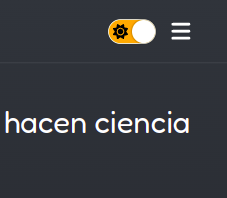
\includegraphics[width=0.3\textwidth]{imagenes/07_Implementacion/menu_oculto.png}}
\subfloat[Estado desplegado]{
\label{subfig:menu_desplegado}
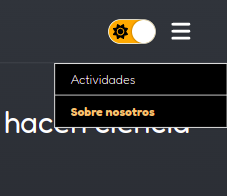
\includegraphics[width=0.3\textwidth]{imagenes/07_Implementacion/menu_desplegado.png}}
\caption{Estados del menú lateral}
\label{fig:estados_menu_lateral}
\end{figure}

\section{Inclusión de las ventanas emergentes en el sistema} \label{sec:inclu_ventanas_emer}

El lenguaje Javascript tiene por defecto órdenes para crear ventanas emergentes, pero estas ventanas tienen un estilo muy básico. Para tener ventanas emergentes con un estilo interesante para el usuario se ha utilizado el plugin SweetAlert2. En su página oficial \footnote{\url{https://sweetalert2.github.io}} se muestran varios ejemplos de usos de este plugin. Para la creación de mis ventanas me he basado en varios de estos ejemplos. Para empezar a poder usar este plugin es necesario incluir en el archivo HTML de la página donde se quiera usar, un enlace a los archivos que forman el plugin.

Todas las ventanas disponen de una serie de atributos \footnote{\url{https://sweetalert2.github.io/#title}}, los cuales pueden ser definidos o no. Entre ellos podemos encontrar el título de la ventana, el color de los botones, y muchos más.

Para lanzar la ventana y que se haga visible, se emplea la función \textit{Swal.fire}\ . Pero aquí no queda la cosa porque existen ventanas que dan solamente información, y otras que dan información y esperan una interacción del usuario; lo interesante de estas últimas es que se debe gestionar la respuesta del usuario. Esta gestión se realiza en el \textit{then} de la función \textit{Swal.fire}, el cual se activa cuando esta función devuelve una \textit{Promise}.

La información que se suele gestionar es la indicación de que botón ha pulsado el usuario. Para ello, este plugin dispone de funciones que nos facilitan conocer esta información, las cuales se pueden comprobar en su página oficial en el apartado "Handling buttons".

Hasta este momento se puede tener una idea de como funcionan estas ventanas emergentes. Falta explicar como las hemos utilizado en nuestro sistema. En nuestro caso hemos creado tres ventanas emergentes distintas. Todas las ventanas originadas hacen uso del botón de confirmación y de cancelación. Estas ventanas se describen a continuación:

\begin{itemize}
\item \textbf{Permiso para la toma de imágenes:} Esta ventana se lanza al pulsar sobre alguno de los botones que abre el chatbot en alguno de los canales disponibles. Estos botones se pueden ver en la Figura \ref{fig:botones_canales}.

\begin{figure}[h]
\centering
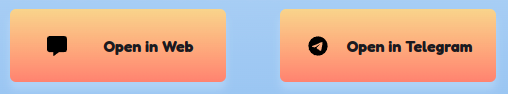
\includegraphics[width=0.7\textwidth]{imagenes/07_Implementacion/botones_canales.png}
\caption{Botones para el acceso a los canales de comunicación con el chatbot}
\label{fig:botones_canales}
\end{figure}

La ventana emergente informa al usuario de que la deducción de la edad se va a producir a través de una imagen, y, por lo tanto, si quiere o no que se le tomen imágenes. Además, se indica que no se puede revertir la decisión. Esta ventana se puede ver en la Figura \ref{fig:popup_pemisos}.

En el caso de que el usuario confirme la toma de imágenes, se abrirá la sección de captura de imágenes. En caso contrario, al negar la toma de imágenes por parte del usuario se lanzará una nueva ventana emergente.

Este punto de decisión puede parecer innecesario si leemos la función de la siguiente ventana emergente, donde se decide de forma explícita por parte del usuario su edad. Pero esta opción de deducir la edad a través de las imágenes está pensada como una funcionalidad a futuro, ya que si nuestro sistema evoluciona pasando de un entorno estático a un entorno en movimiento, esta manera de deducir la edad sería ideal para adaptar nuestro sistema a este nuevo entorno. Por esta razón se ha incluido este punto de decisión para poder darle más posibilidades a futuro a nuestro sistema.

\item \textbf{Indicación explícita de la edad:} Esta ventana emergente es la que se genera en caso de negar la toma de imágenes en la ventana emergente del punto anterior. En esta ventana se preguntará explícitamente la edad del usuario. Y además, aparecerán exactamente dos rangos de edad: Niño o Adulto. Esta ventana se puede ver en la Figura \ref{fig:popup_edad}. Cuando el usuario elige alguno de los dos rangos de edad, se abrirá la interfaz del chatbot a través del canal que haya elegido el usuario cuando pulsó el botón que lanzó la primera ventana emergente.

\begin{figure}
    \centering
    \subfloat[Ventana emergente para la adquisición de permisos de toma de imágenes]{
    \begin{subfigure}
        \centering
        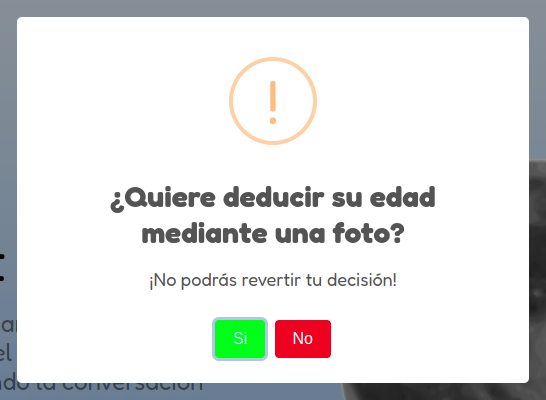
\includegraphics[width=0.4\textwidth]{imagenes/07_Implementacion/popup_permisos.png}
        \label{fig:popup_pemisos}
    \end{subfigure}
    }
    \hspace{5mm}
    \subfloat[Ventana emergente para la deducción de la edad]{
    \begin{subfigure}
        \centering
        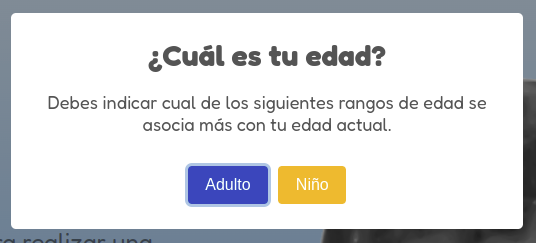
\includegraphics[width=0.4\textwidth]{imagenes/07_Implementacion/popup_edad.png}
        \label{fig:popup_edad}
    \end{subfigure}
    }
    \hfill
    \subfloat[Ventana emergente para la adquisición de permisos de envío de imágenes]{
    \begin{subfigure}
        \centering
        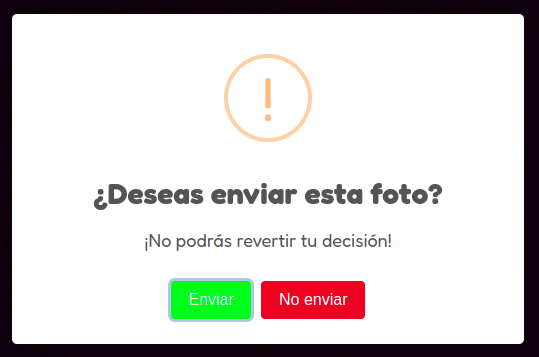
\includegraphics[width=0.5\textwidth]{imagenes/07_Implementacion/popup_enviar.png}
        \label{fig:popup_enviar}
    \end{subfigure}
    }
\caption{Ventanas emergentes de la Vista}
\end{figure}


\item \textbf{Permiso para el envío de la imagen tomada:} Esta ventana se lanza al pulsar sobre el botón de ``Enviar'' (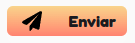
\includegraphics[width=0.15\textwidth]{imagenes/07_Implementacion/boton_enviar.png}) situado en la sección de captura de imágenes, el cual aparece una vez se ha capturado la imagen; y también se lanza cuando en el caso del móvil, se acepta enviar la imagen desde la aplicación de captura de imágenes del sistema. Esta última forma depende del dispositivo que se esté utilizando porque depende de la aplicación del sistema.

La ventana emergente informa al usuario de que se va a producir el envío de la imagen tomada por el dispositivo de captura, y, por lo tanto, si quiere o no que se realice el envío de la imagen en cuestión. Además, se indica que no se puede revertir la decisión, ya que al decidir no enviar la imagen se cierra la ventana emergente. Esta ventana se puede ver en la Figura \ref{fig:popup_enviar}.

En el caso de que el usuario confirme el envío de imágenes, se procederá a efectuar el envío de la imagen para su posterior análisis para deducir la edad del usuario. Durante el tiempo que dure el envío de la imagen y su análisis se mostrará una figura de carga para proporcionar feedback al usuario. En caso contrario, al negar el envío de la imagen por parte del usuario, se procederá a cerrar la ventana emergente y a esperar a que el usuario vuelva a tomar una imagen que le parezca adecuada y vuelva a iniciar el proceso de envío de la imagen.

\end{itemize}


\section{Inclusión de la interfaz web de Dialogflow en el sistema} \label{sec:inclu_interfaz_web}

Para obtener esta interfaz web debemos acceder al chatbot que hemos creado en Dialogflow. En nuestro caso hemos generado un agente por cada rango de edad. Lo hemos hecho de esta forma para diferenciar con que agente está charlando el usuario, ya que como hemos indicado anteriormente, al emplear una interfaz que no es nuestra, perdemos parte del control y en consecuencia, si tenemos un agente único, no podremos diferencia los mensajes de un usuario del rango de Adulto, de los mensajes de un usuario del rango de Niño.

Una vez nos encontramos dentro del agente en Dialogflow, nos dirigimos al apartado de Integrations, el cual se puede ver en la Figura \ref{fig:integrations_dialogflow}.

\begin{figure}[h]
\centering
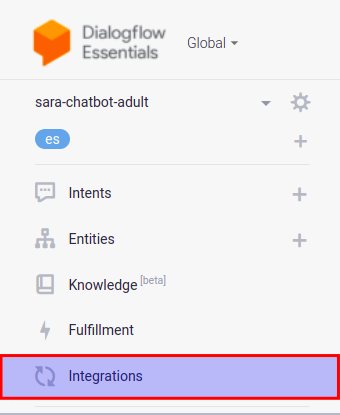
\includegraphics[width=0.4\textwidth]{imagenes/07_Implementacion/integrations_dialogflow.png}
\caption{Apartado Integrations de un agente de Dialogflow}
\label{fig:integrations_dialogflow}
\end{figure}

Dentro de este apartado nos dirigimos a la sección Text based donde se encuentra Web Demo, que es la interfaz web de Dialogflow. Este apartado se puede ver en su totatilidad en la Figura \ref{fig:text_based}.

\begin{figure}[h]
\centering
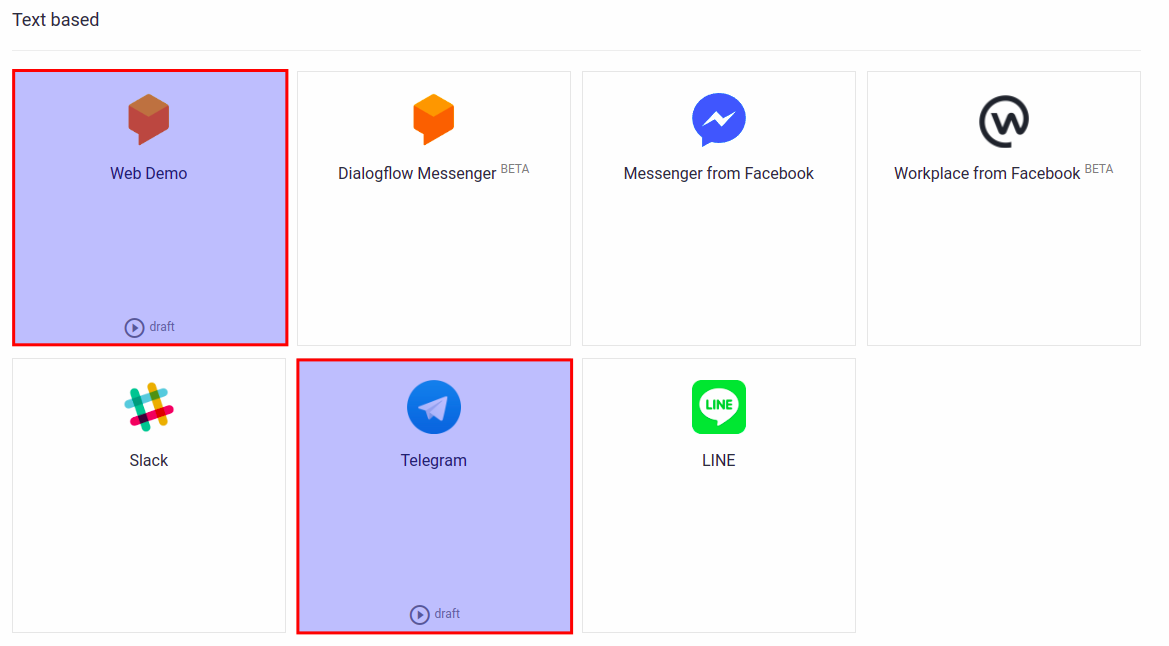
\includegraphics[width=0.6\textwidth]{imagenes/07_Implementacion/text_based.png}
\caption{Sección Text based del apartado Integrations}
\label{fig:text_based}
\end{figure}

Al pulsar sobre Web Demo aparece una ventana emergente donde se puede habilitar esta interfaz para el chatbot que se esté utilizando. Esta ventana emergente se puede ver en la Figura \ref{fig:web_demo}. Una vez habilitada se podrá hacer uso de ella mediante un iframe. Este iframe al colocarlo en un archivo HTML, incrustará el código HTML de la interfaz web de Dialogflow.

\begin{figure}[h]
\centering
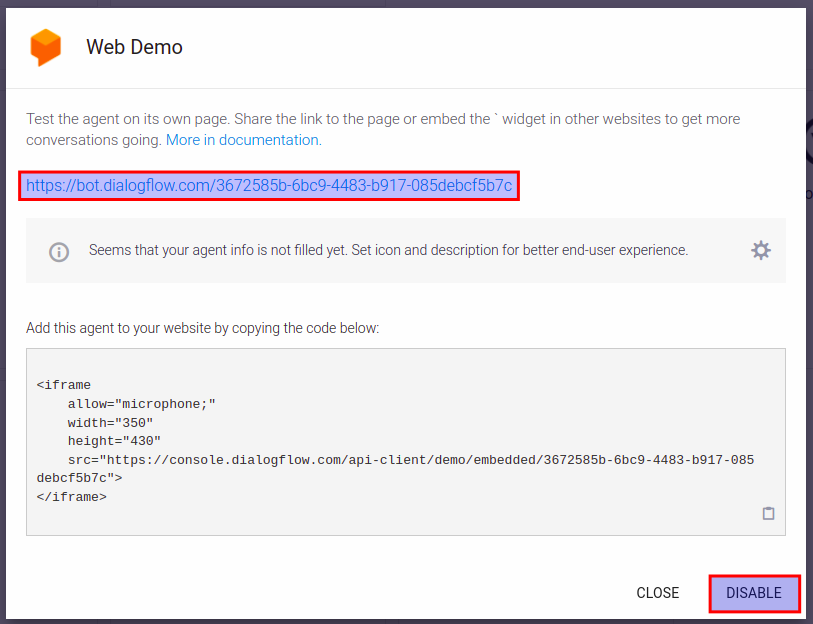
\includegraphics[width=0.7\textwidth]{imagenes/07_Implementacion/web_demo.png}
\caption{Ventana emergente de Web Demo de Dialogflow}
\label{fig:web_demo}
\end{figure}

Para obtener el código del iframe se accede a la URL que aparece marcada en la Figura \ref{fig:web_demo}. Al abrir esta URL nos abrirá una nueva ventana donde se puede ver el código del iframe del chatbot donde nos encontremos. Esta ventana se puede ver en la Figura \ref{fig:dialogflow_iframe}.

\begin{figure}[h]
\centering
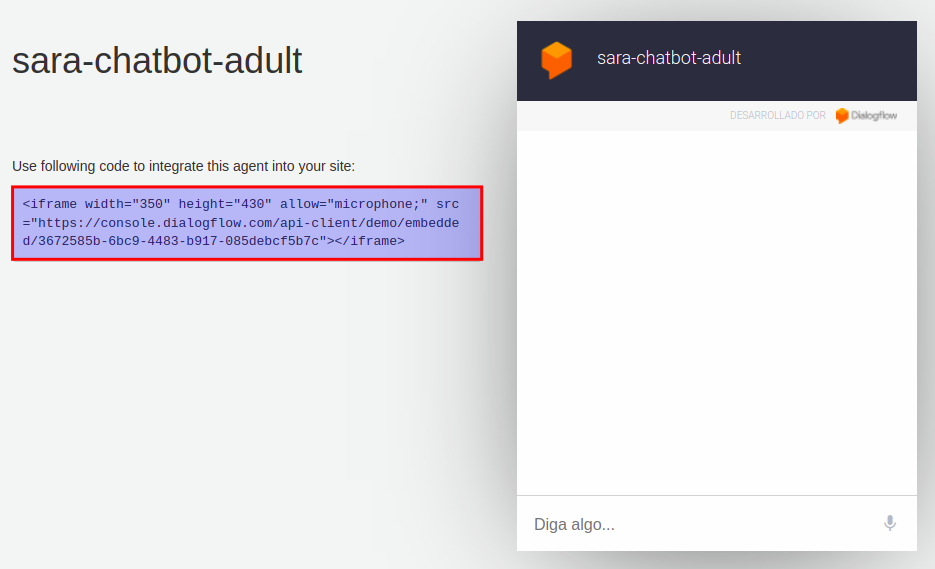
\includegraphics[width=0.7\textwidth]{imagenes/07_Implementacion/dialogflow_iframe.png}
\caption{Ventana donde se muestra el código del iframe}
\label{fig:dialogflow_iframe}
\end{figure}

El código del iframe de uno de los chatbots creados en Dialogflow se puede ver en la Figura \ref{fig:codigo_iframe}. Como se puede apreciar se indica el tamaño de ventana que tendrá la interfaz. Para que la interfaz se adapte al tamaño que nosotros le indiquemos en nuestro sitio web, se eliminan estos dos atributos del iframe. El siguiente atributo que aparece son los permisos que necesita la interfaz web. Como se puede ver se indica el micrófono, ya que además de poder introducir texto de forma escrita, también se puede introducir de forma oral; pero para ello es necesario que el usuario de permisos para el uso del micrófono por parte de nuestro sitio web. Y por último, el atributo que aparece al final es la dirección al código de la interfaz web, el cual será integrado en nuestro sitio web.

\begin{figure}[h]
\centering
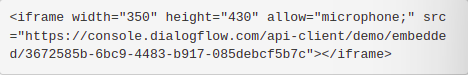
\includegraphics[width=0.7\textwidth]{imagenes/07_Implementacion/codigo_iframe.png}
\caption{Código del iframe del chatbot para adultos}
\label{fig:codigo_iframe}
\end{figure}

El aspecto final de nuestra interfaz web se puede ver en la Figura \ref{fig:interfaz_web}.

\begin{figure}[h]
\centering
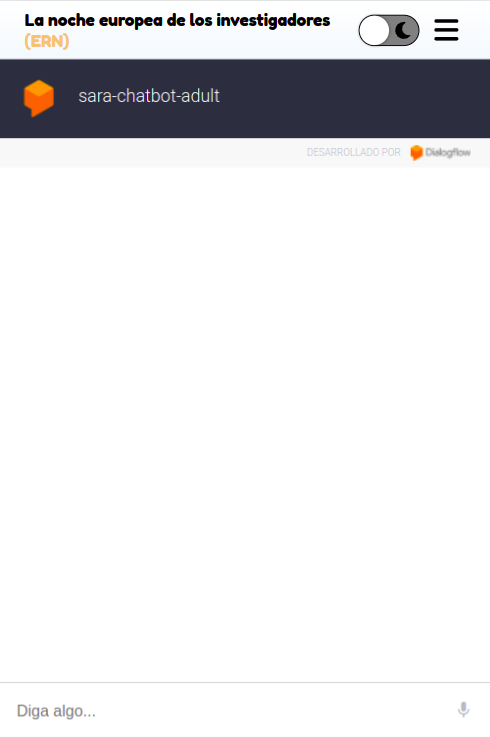
\includegraphics[width=0.4\textwidth]{imagenes/07_Implementacion/interfaz_web.png}
\caption{Aspecto de la interfaz web del chatbot para adultos desde una tablet en orientación vertical}
\label{fig:interfaz_web}
\end{figure}


\section{Inclusión de la interfaz de Telegram de Dialogflow en el sistema} \label{sec:inclu_interfaz_telegram}

Para obtener la interfaz de Telegram primeramente debemos acceder a la sección de Telegram dentro del apartado de Integrations de Dialogflow, que se puede ver en la Figura \ref{fig:text_based}. Al pulsar en la sección de Telegram, aparecerá una ventana emergente parecida a la de Web Demo, donde se solicita el token del chatbot. Se solicita un token porque todos los bots en Telegram tienen asignado un token. Esta ventana emergente se puede ver en la Figura \ref{fig:token_telegram}.

\begin{figure}[h]
\centering
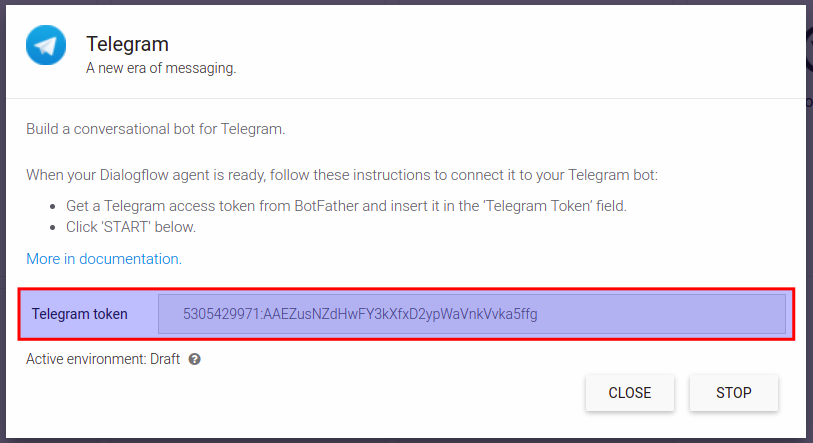
\includegraphics[width=0.6\textwidth]{imagenes/07_Implementacion/token_telegram.png}
\caption{Ventana emergente de Telegram de Dialogflow}
\label{fig:token_telegram}
\end{figure}

Por lo que llegados a este punto debemos crear un bot en la aplicación de Telegram, para poder hacer uso de él como interfaz para nuestro chatbot. Para generar un chatbot en Telegram se debe acceder a BotFather, que es un bot cuyo objetivo es la creación del resto de bots que existen en Telegram. El chat con este bot se puede ver en la Figura \ref{fig:bot_father}.

\begin{figure}[h]
\centering
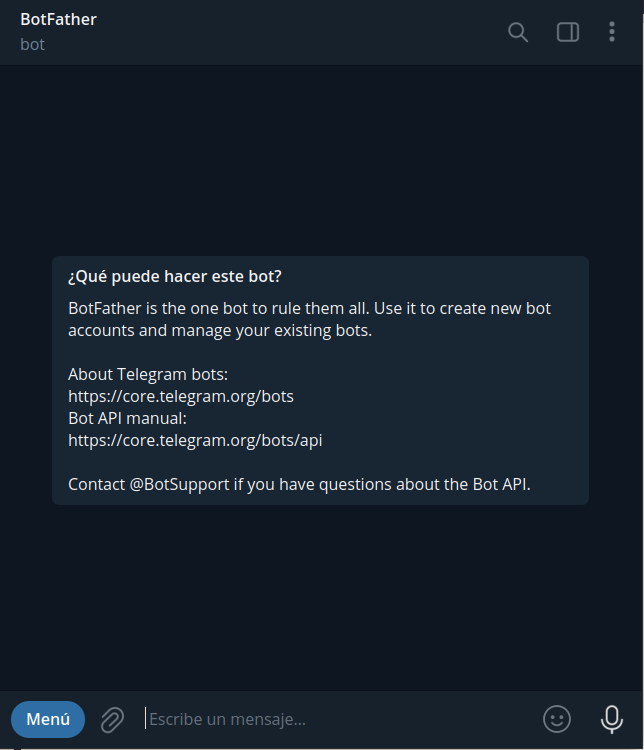
\includegraphics[width=0.4\textwidth]{imagenes/07_Implementacion/bot_father.png}
\caption{Chat con el bot de Telegram BotFather}
\label{fig:bot_father}
\end{figure}

Con el comando /newbot se inicia el proceso de creación del bot. Durante este proceso se nos solicita el nombre del bot; y posteriormente se nos solicita el username del bot, el cual debe terminar con la palabra "bot" o "Bot". Una vez terminado este proceso aparecerá un mensaje con el token asociado a nuestro nuevo bot. De la misma forma que para la interfaz web se producen dos chatbots en Dialogflow, para la interfaz de Telegram también se deben crear dos bots y obtener los tokens de ambos.

Una vez tenemos este token lo introducimos tal y como aparece en la Figura \ref{fig:token_telegram}.

El aspecto final de nuestra interfaz de Telegram será el que se muestra en la Figura \ref{fig:interfaz_telegram}.

\begin{figure}[h]
\centering
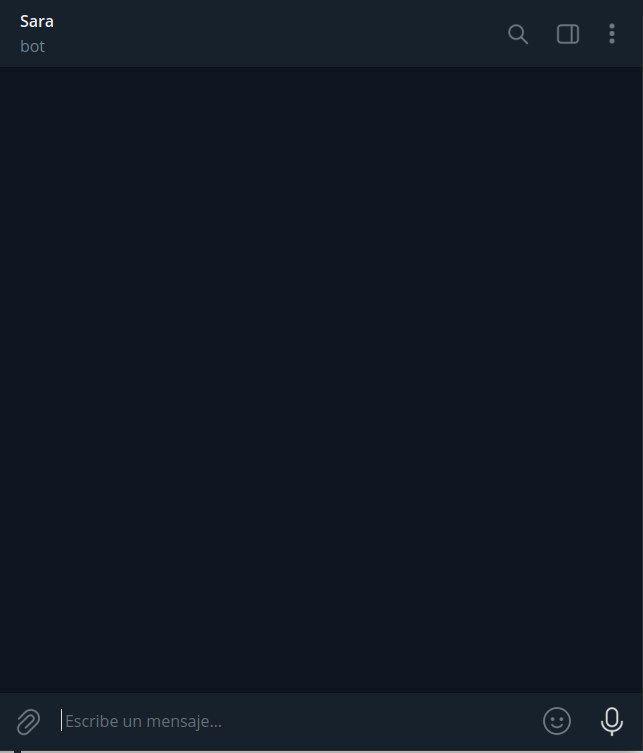
\includegraphics[width=0.4\textwidth]{imagenes/07_Implementacion/interfaz_telegram.png}
\caption{Aspecto de la interfaz de Telegram del chatbot para adultos}
\label{fig:interfaz_telegram}
\end{figure}


\section{Razones adicionales de la elección del framework para el servidor} \label{sec:razones_framework_server}

Por supuesto, existe una gran cantidad de frameworks basados en Python para la elaboración de API's, pero como se puede ver en la Figura \ref{fig:comparativa_fastapi}, donde se compara el rendimiento de distintos frameworks. El framework FastAPI es el que obtiene unos mejores resultados entre los frameworks basado en Python, de ahí su elección para nuestro servidor, ya que queremos que las peticiones al servidor se gestionen lo más rápido posible para agilizar la comunicación con el chatbot y el movimiento por el sitio web.

\begin{figure}[h]
\centering
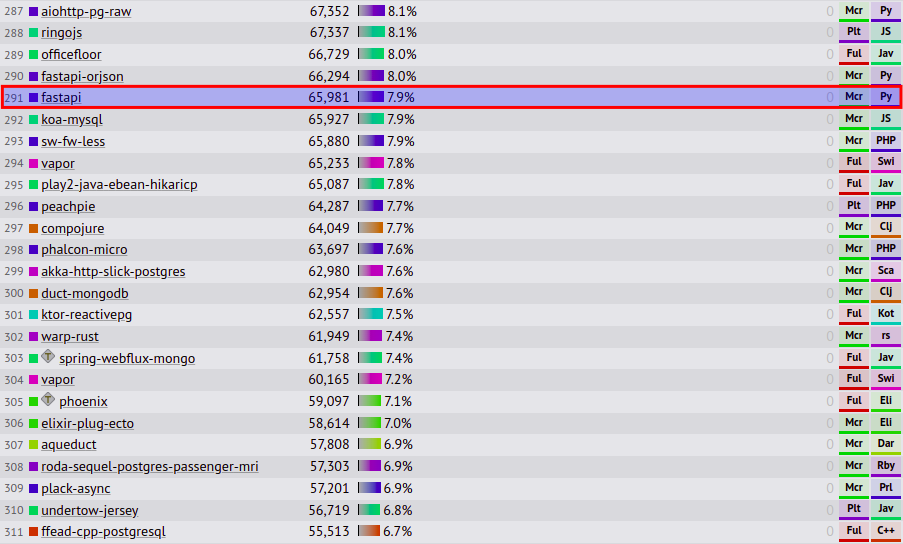
\includegraphics[width=0.8\textwidth]{imagenes/07_Implementacion/comparativa_fastapi.png}
\begin{center}
Fuente: \url{https://www.techempower.com/benchmarks/#section=data-r20&hw=ph&test=db}
\end{center}
\caption{Número de respuestas por segundo para peticiones (Datos del 02/08/2021)}
\label{fig:comparativa_fastapi}
\end{figure}


\section{Despliegue del servidor en Heroku} \label{sec:proce_despli_server_Heroku}

El despliegue a la plataforma Heroku se puede efectuar por tres vías. Una vez que creamos nuestra app en la plataforma de Heroku, si accedemos a la misma y nos vamos a la sección Deploy, podremos ver las tres vías que existen. Estas vías se pueden ver en la Figura \ref{fig:deploy_heroku}.

\begin{figure}[h]
\centering
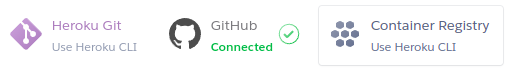
\includegraphics[width=0.7\textwidth]{imagenes/07_Implementacion/deploy_heroku.png}
\caption{Métodos de despliegue de apps en Heroku}
\label{fig:deploy_heroku}
\end{figure}

En mi caso he optado por el tercer método, el cual involucra a los contenedores. Por esta razón se menciona en anteriores párrafos el uso de Docker, ya que se efectuará el despliegue de la app como un contenedor. Las ventajas de los contenedores son que producen una menor sobrecarga, permiten una mayor portabilidad, y son más eficientes, entre muchos otros.

Los pasos a seguir siguiendo este método se explican en el apartado Container Registry \footnote{\url{https://dashboard.heroku.com/apps/sara-chatbot-tfg/deploy/heroku-container}} de la sección Deploy de la app. Los únicos requisitos para este método es tener instalado en el sistema tanto Heroku CLI como Docker.

Pero yo he seguido una vía alternativa, dado que estamos usando Github como plataforma para el control del código del proyecto, he optado por sacar potencial a la funcionalidad de los Workflows que se nos proporciona en Github. Estos Workflows no son más que procesos automatizados que se pueden configurar con uno o más trabajos. Para la creación de los archivos que componen a estos Workflows se hace empleo del lenguaje YAML.

Basándonos en estos Workflow he configurado un trabajo que realiza el despliegue del Controlador en la plataforma Heroku de forma automática cuando se percibe por parte de Github que ha habido cambios en el código del Controlador.

Además, para una mayor capacidad de configuración se ha hecho uso de los Actions secrets de Github. Esta funcionalidad de Github permite guardar valores en variables que puede ser utilizadas desde los trabajos de los Workflows, y siendo además privados, por lo que se pueden guardar datos sensibles como contraseñas.

Siguiendo con el trabajo que efectúa el despliegue del Controlador, este trabajo se podría haber implementado en su totalidad por mí, pero para ahorrar tiempo y evitar errores que pudiesen surgir he optado por usar un Action creado por otra persona. Los trabajos de los Workflows se componen de una serie de Actions. El Action utilizado pertenece a AkhileshNS y se llama \href{https://github.com/AkhileshNS/heroku-deploy}{heroku-deploy}. Para facilitar el uso de este Action se dispone de ejemplos de uso en su repositorio de Github. Los datos que requiere este Action para realizar el despliegue es la API key de nuestra cuenta de Heroku, el nombre que le hemos asignado a nuestra app a la hora de generarla en Heroku, en nuestro caso es sara-chatbot-tfg, el email empleado a la hora de registrarnos en la plataforma de Heroku, y por último el directorio donde se encuentra el Dockerfile que define al contenedor. Los tres primeros datos estarán guardados en tres variables distintas dentro de los Actions secrets de nuestro repositorio de GitHub, donde se controla el código de nuestro proyecto.

Hasta este punto tenemos una forma de efectuar el despliegue automático, pero necesitamos definir como debe formarse el contenedor. Como se ha indicado en el anterior párrafo, al Action es necesario indicarle donde se encuentra un archivo en concreto, el Dockerfile. Este archivo es vital para la elaboración de un contenedor. Un Dockerfile es un archivo de texto simple que define un conjunto de comandos que se ejecutará para formar el entorno del contenedor. Para generar nuestro contenedor del Controlador hemos usado como base del contenedor una imagen de Python cuya versión es 3.9.10\ . Posteriormente, se copia todo el contenido del directorio, incluido el propio directorio, que contiene todo el código del Controlador en la raíz del contenedor. Después de realizar la copia se establece como directorio de trabajo el propio directorio que se ha copia en el contenedor. Seguidamente, procedemos a la instalación de los requisitos del Controlador mediante el comando pip. Y finalmente, establecemos como punto de entrada al contenedor la ejecución del script main.py, el cual ejecutará el inicio del servidor del Controlador.

Después de todos lo dicho ya tendríamos un servidor para el Controlador al que se puede acceder de forma pública y en cualquier momento.

Aunque el trabajo que efectúa el despliegue no es el único que he elaborado relacionado con el Controlador, ya que puesto que estamos usando contenedores para realizar el despliegue, pensé que era buena idea subir el contenedor que se obtiene con el controlador a la plataforma DockerHub \footnote{\url{https://hub.docker.com}}. Esta plataforma es el equivalente a GitHub para contenedores, sirve como plataforma para albergar contenedores en repositorios privados o públicos. Esta subida se hace con otro trabajo dentro del mismo Workflow del despliegue del Controlador para aprovechar la automatización lograda. El único requisito para proceder a la subida es tener instalado en la máquina el paquete Docker. Una vez lo tenemos instalado la subida consiste en los siguientes pasos:

\begin{itemize}
\item Login en la plataforma de DockerHub con nuestro usuario y contraseña
\item Construcción de la imagen del contenedor
\item Subida de la imagen al repositorio \href{https://hub.docker.com/repository/docker/macarse/sara-chatbot-controller}{sara-chatbot-controller}
\end{itemize}

Ahora, al disponer de la imagen del contenedor en un repositorio, se podría cambiar fácilmente la plataforma donde se despliega siempre y cuando se pueda efectuar el despliegue mediante contenedores.

Llegados a este punto tendríamos una estructura de despliegue del Controlador totalmente automatizada.


\section{Proceso de generación de plantillas renderizadas} \label{sec:proce_gen_plantillas}

Para generar una plantilla renderizada se hace uso del método TemplateResponse del objeto templates. Este método requiere de dos parámetros. El primer parámetro será una cadena con la ruta relativa de la plantilla que se quiere renderizar. Esta ruta relativa tomará como base el directorio que se indicó en la creación del objeto templates, este directorio es el directorio que contiene todas las plantillas del servidor llamado templates. El segundo parámetro será un diccionario donde cada par clave-valor estará compuesto por una cadena que será la clave y por una variable que será el valor. Es importante la cadena que se utilice como clave, ya que con ese nombre se podrá acceder al valor asignado desde el código de las plantillas. Algo relevante a destacar es que al menos este diccionario debe tener un elemento, el cual es el parámetro de tipo Request que se indicó en la lista de pasos.


\section{Paso de la información a los script de Javascript} \label{sec:paso_info_scripts}

Al hacer empleo del diccionario hacemos que esta información únicamente sea accesible desde la plantilla, pero no desde el código Javascript, que es donde realmente es necesaria esta información, ya que es el lugar donde se ejecuta la lógica de las plantillas. Para acceder a la información de una clave se debe escribir en la plantilla de código HTML el nombre de la clave dentro de dos llaves a ambos lados, es decir, si la clave se llama estado para acceder a su valor se debe escribir \{\{estado\}\}. Esta forma de acceder a la información solamente es posible desde el código HTML, en este punto es donde entra en juego el uso del lenguaje HTML dentro de la implementación del Controlador, la cual se mencionó en el apartado de herramientas de desarrollo del Controlador (Apartado \ref{subsec:herramientas_controlador}).

Para poder acceder a esta información desde los scripts de Javascript se creará un párrafo de HTML para cada clave que se pase al diccionario, el cual contendrá la información de esa clave. Este párrafo tendrá un estilo que le otorgue la visibilidad de oculto. Y para acceder a la información se obtendrá el elemento HTML desde el script de Javascript y ya tendremos acceso a esa información. Un ejemplo de definición de un párrafo para una clave se puede ver en la Figura \ref{fig:def_clave_jinja}.

\begin{figure}[h]
\centering
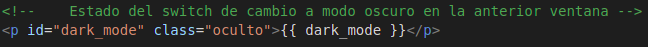
\includegraphics[width=0.8\textwidth]{imagenes/07_Implementacion/def_clave_jinja.png}
\caption{Ejemplo de definición de una clave en una plantilla HTML}
\label{fig:def_clave_jinja}
\end{figure}


\section{Solución a la inactividad de las apps de Heroku} \label{sec:inactividad_Heroku}

Una solución provisional que se suele usar es la ejecución de comandos ping al servidor de manera periódica. Para la ejecución periódica de estos comandos se hace empleo de la plataforma \href{https://console.cron-job.org/}{cron-job}. Dentro de esta plataforma se pueden crear trabajos que se ejecutan cada cierto tiempo, tiempo que se puede definir en el trabajo. Estos trabajos ejecutan un comando ping a la dirección URL que se le indique en el trabajo. Para gestionar estos ping al servidor se ha generado la sección wakeup en el servidor del Controlador. A esta sección será a la que se realicen los comandos ping. Esta sección lo único que hace es devolver un texto plano indicando el estado activo del servidor.

\section{Proceso para la gestión de la conversación desde el Controlador} \label{sec:proce_gestion_conver}

La gestión de la petición de Dialogflow por parte del Controlador se efectúa de manera similar independientemente del rango de edad, el único cambio es que la respuesta se obtiene efectuando la llamada a secciones distintas del servidor del Modelo. La gestión de la petición comienza obteniendo el Intent que lanzó la petición, ya que según el Intent se realizan algunos pasos distintos. El chatbot tendrá dos Intents, el Intent Talk y el Intent Goodbye. En el Intent Talk se efectúa toda la conversación, excepto la última interacción con el chatbot, que se realiza en el Intent Goodbye.

Si se trata del Intent Talk, el siguiente paso será comprobar si se trata de la primera generación de respuesta o no. Para obtener esta información se revisa el contexto que contiene la petición. Si dentro del contexto está el campo edad quiere decir que no es la primera respuesta, en caso contrario indica que si se trata de la primera respuesta.

Cuando se trata de la primera generación de respuesta, primeramente se verifica si el servidor del Modelo se encuentra activo. Si no se encuentra activo se le indica al usuario mediante una respuesta a través del chatbot. Si se encuentra activo, se extrae la información necesaria del contexto de la petición para efectuar la generación de la respuesta. Esta información es el texto de entrada y la edad, la cual se deduce de forma sencilla al ver a que webhook ha llegado la petición. Una vez se ha generado la respuesta, se elaborará el primer contexto de la conversación. Para la elaboración de este primer contexto será necesario obtener la fecha actual, que marcará el inicio de la conversación. Al contexto se añadirá la información de la fecha de inicio, la edad del usuario, se incluirá la entrada y la salida que se ha generado a partir de esa entrada y finalmente se añadirá el identificador de la conversación, el cual es muy importante para seguir la conversación en el resto de llamadas al webhook. La respuesta a la petición del webhook estará compuesta por el texto que se ha generado como respuesta al texto de entrada, y por el nuevo contexto que se ha generado.

Cuando se trata del resto de generaciones de respuestas, habrá pasos que se eviten sustituyéndolos por otros. En este caso, a la hora de generar la respuesta será necesario, el texto de entrada, al igual que pasaba en el otro caso; la edad, que en este caso se extraerá del contexto de la petición; y el identificador de la conversación, para indicar al Modelo de que se trata de una respuesta que continúa una conversación ya empezada. La generación del contexto evitará el añadir la fecha de inicio y la edad, ya que fueron añadidos en la primera generación. En esta generación de contexto solamente se añadirá el texto de entrada y la respuesta a la misma, y se actualizará el identificador de la conversación. La respuesta a la petición del webhook se elaborará de la misma forma.

Una vez hemos detallado el proceso con el Intent Talk. Si se trata del Intent Goodbye, los pasos a seguir son exactamente iguales a los realizados con el Intent Talk cuando no es la primera generación, con la única salvedad de que al final de todos los pasos se guardará la conversación en el log del sistema, para poder utilizar esta información para futuras mejoras del chatbot y también para el análisis de las conversaciones que se han realizado con el chatbot. El contexto no se guarda tal cual en el log, sino que más bien se formatea la información del contexto para guardarla de una manera clara en ella. Cabe destacar que antes de guardar la conversación se debe obtener la fecha actual para usarla como la fecha de finalización de la conversación. El guardado de la conversación en el log se explica en el Apartado \ref{subsec:guardado_conver}.

La generación de la respuesta consistirá en el envío de una petición al servidor del Modelo. La petición se enviará a la sección del servidor del Modelo acorde con la edad que se haya indicado a la función de generación de respuestas. Esta petición contendrá como información el texto de entrada, el identificador de la conversación en caso de conocerse, y un indicador de si es la última respuesta, información que es útil para el Modelo para su propia gestión de las conversaciones. La respuesta se obtendrá de la respuesta a esta petición al servidor del Modelo.

El contexto que se encuentra dentro de la petición al webhook está compuesto de varios elementos, ya que un chatbot en Dialogflow puede tener un contexto compuesto de varios elementos, donde cada elemento tenga cierta información. Pero para nuestro chatbot toda la información se guardará en el mismo elemento. El contexto donde se guardará toda la información será el llamado \textit{talk-followup}.


\section{Establecimiento de la conexión entre el servidor y el log} \label{sec:conexion_server_log}

Para efectuar la conexión se sigue la documentación de Heroku relaciona con la conexión del log con Python \footnote{\href{https://devcenter.heroku.com/articles/connecting-heroku-postgres#connecting-in-python}{https://devcenter.heroku.com/articles/connecting-heroku-postgres}}. En primer lugar, será necesario tener instalada la librería \textit{psycopg2-binary}. Dentro del código del servidor se hará import de la librería para poder acceder al log de la app. El primer paso para acceder al log, es la conexión con la misma. La conexión se realiza mediante la función connect de la librería. Esta función requiere de la URL del log, la cual se puede obtener mediante las variables de configuración de nuestra app. Esta función devolverá un objeto que representará la conexión con el log. Una vez hemos efectuado la conexión, debemos ver como escribir los datos de la conversación en el log, para ello es necesario obtener el cursor del log. Con este cursor se podrán ejecutar comando SQL sobre el log utilizando los datos de la conversación. Antes de realizar la escritura de los datos se deberán obtener las conversaciones con un formato claro, para facilitar su análisis en el log. Finalmente, cuando tenemos todos los datos listos, ejecutamos un comando INSERT sobre la tabla que contendrá las conversaciones. Este comando insertará la edad del usuario, la fecha de inicio de la conversación, la fecha de finalización de la misma y el contenido de la conversación, es decir, las distintas entradas y salidas de la conversación.

Cuando ya hemos insertado los datos en la tabla debemos comunicar al log los cambios mediante la función \textit{commit}. De esta forma, los cambios se harán permanentes en el log. Llegados a este punto ya hemos terminado el guardado de la conversación, por lo tanto, ya podemos cerrar tanto el cursor como el log. Ambos cierres se realizan con la función \textit{close} aunque sobre distintos objetos.


\section{Cabeceras añadidas a las conexiones con el servidor del Modelo} \label{sec:cabecera_conexion_Modelo}

Estas cabeceras son las llamadas cabeceras CORS o cabeceras de Intercambio de recursos de origen cruzado. Dado que para la implementación del servidor se hace uso del framework FastAPI, utilizaremos las herramientas que nos proporciona este framework para solucionar este problema. La herramienta a utilizar en este caso es la adhesión de un middleware de tipo CORS, para ello se debe hacer uso de la función \textit{add\_middleware} y de la clase \textit{CORSMiddleware}. Como se indica en \href{https://fastapi.tiangolo.com/tutorial/cors/}{la documentación de FastAPI}, este tipo de middleware se utiliza en situaciones en las que la interfaz tiene código Javascript que se comunica con un backend y el backend está en un dominio diferente al de la interfaz.


\section{Proceso de despliegue del servidor del Modelo mediante Ngrok} \label{sec:proce_despli_server_Modelo}

Por supuesto, antes de nada es necesario importar la librería pyngrok, así como instalar ngrok en el sistema donde se ejecutará el servidor para poder generar la conexión entre el servidor e internet. 
 
 En primer lugar, deberemos definir la configuración del túnel que se originará. Esta configuración se guardará en un archivo de tipo YAML. Dentro de este archivo encontraremos la siguiente información:

\begin{itemize}
\item Token de autenticación de Ngrok
\item Región de la conexión
\end{itemize}

El token de autenticación se puede extraer de la sección Your Authtoken de nuestra cuenta en la plataforma de Ngrok.

Esta configuración se definirá en el código mediante la clase PyngrokConfig. Esta clase necesita de dos elementos para poder crear una instancia. Por un lado, la ruta al ejecutable de ngrok que se ha generado al realizar la instalación de ngrok en el sistema; y, por otro lado, la ruta al archivo de configuración anteriormente descrito.

Finalmente, se efectuará la conexión, obteniendo la URL pública del servidor. Para realizar la conexión se hará uso de la configuración definida anteriormente y del puerto utilizado para ejecutar el servidor, el cual es el mismo que se utilizó con el módulo Uvicorn. Llegados a este punto habremos efectuado la conexión y dispondremos de un servidor para el Modelo totalmente funcional y accesible.

Pero si nos fijamos la forma de desplegar el servidor del Modelo, causa que tengamos una URL pública distinta cada vez que iniciamos o reiniciamos el servidor, a diferencia de lo que pasa con el servidor del Controlador que tiene una URL pública fija al emplear la plataforma Heroku para su despliegue. Esta condición del servidor del Modelo provoca la creación de una funcionalidad que comparta la URL del servidor del Modelo con el servidor del Controlador. Para ello se ha creado una función que envía la URL pública almacenada en el servidor del Modelo a través de una petición POST con destino a la sección para fijar la URL del servidor del Controlador, la cual fue descrita en la implementación del Controlador. La petición POST contendrá la URL pública del servidor del Modelo.

Esta función se ejecutará junto al código que arranco la ejecución del servidor. Además, se creará una sección en el servidor del Modelo, cuya funcionalidad consista en volver a enviar la URL al servidor del Controlador a pesar de haber inicio el servidor. La finalidad de esta sección es volver a conectar ambos servidores cuando sea el servidor del Controlador el que se reinicie mientras el servidor del Modelo siga activo.

Un tip que puede ser útil para la gestión de las conexiones con Ngrok, es el uso del comando \textit{killall ngrok}. Este comando elimina todas las conexiones establecidas actualmente mediante Ngrok. Puede llegar a ser útil si el servidor del Modelo finaliza de forma inesperada y no es capaz de finalizar el proceso que ejecuta el servidor adecuadamente. Este problema surge sobre todo cuando se utiliza la versión gratuita de Ngrok, ya que solamente se dispone de una conexión disponible.


\section{Preprocesado de los conjuntos de datos} \label{sec:preprocesado_conj_datos}

El primer paso en el pre procesado es la obtención de los conjuntos de datos para cada rango de edad a partir del conjunto de datos inicial. En primer lugar, se realiza una resumen de todos los textos del conjunto de datos, ya que vamos a implementar un chatbot que tenga respuestas cortas o medianas, pero que no sean excesivamente largas. Este resumen se efectuará con un modelo basado en Transformers extraído de Huggingface. El modelo empleado es \href{https://huggingface.co/google/pegasus-xsum}{pegasus-xsum} de la empresa Google. Una vez tenemos los textos resumidos, llega el momento de obtener textos diferentes según el rango de edad. Para el caso de los textos para adultos no se hará ninguna modificación adicional, mientras que para los textos para niños si será necesaria una transformación. Dado que los niños tiene una menor capacidad de comprensión, los textos deberán sufrir un proceso de simplificación. Esta simplificación se llevará a cabo mediante modelos preentrenados usados en los experimentos Multilingual Unsupervised Sentence Simplification (MUSS). El código de estos modelos se encuentra en un \href{https://github.com/facebookresearch/muss}{repositorio} de Github de Meta Research. Dentro de este repositorio existen cuatro modelos, pero no todos utilizan texto en inglés. El modelo que he utilizado para mi proyecto es \textit{muss\_en\_wikilarge\_mined}. Tras realizar la simplificación, tendremos todo lo necesario como para obtener dos conjuntos de datos, cada uno orientado a un rango de edad.

El segundo paso del pre procesado es la unión de cada uno de estos conjuntos de datos orientados al rango de edad con un conjunto de datos que contiene información general que será útil para ambos modelos, como puede ser el nombre del chatbot.

Finalmente, el último paso del pre procesado consistirá en dar el formato adecuado a los dos conjuntos de datos generados para que puedan ser usados para el entrenamiento de nuestros modelos. En primer lugar, se deberán dividir ambos conjuntos de datos en sus correspondientes partes de entrenamiento y de validación. Y a su vez, todos los conjuntos de datos generados de esta división deberán reducir sus columnas, dejando únicamente las columnas de Question y de Answer. Además, estas columnas se renombrarán como source y target respectivamente, para que los conjuntos de datos puedan ser empleados en el proceso de ajuste de los modelos.

\section{Extracción de información de Quora} \label{sec:extraccion_info}

Para la extracción de información se va a utilizar el módulo Selenium, el cual tiene implementación en Python. Selenium es un conjunto de utilidades que se emplean para la elaboración de pruebas de aplicaciones web. En nuestro caso usaremos este módulo para recorrer la página de Quora de tal forma que vayamos extrayendo la información que necesitemos de la misma. Selenium puede usar varios navegadores para realizar las pruebas. En el caso de nuestro programa se utilizará el navegador Chrome. Para poder emplear este navegador necesitamos descargar los \href{https://sites.google.com/chromium.org/driver/downloads?authuser=0}{drivers} acordes con nuestra versión de navegador que tengamos instalada en el sistema. En mi caso, la versión de Chrome utilizada es la 101.0.4951.64. Esta información se puede comprobar en la sección de Información de Chrome de la configuración del navegador \footnote{\url{chrome://settings/help}}. La implementación de este programa extractor de información no ha sido fácil debido a la forma en que está estructura la página, ya que se hace poco uso del campo id en los distintos elementos de la página.

Los parámetros que recibirá el programa son los siguientes:

\begin{itemize}
\item Usuario de la cuenta en Quora
\item Contraseña de la cuenta en Quora
\item Número máximo de preguntas a extraer de cada tema
\item Ruta al archivo que contiene las URL's hacia los temas sobre los que extraer información
\item Ruta del archivo que guardará toda la información extraída
\end{itemize}

El formato que tendrán los datos extraídos, los cuales se guardarán en el archivo indicado en la anterior lista, estará compuesto por cuatro columnas. Las columnas serán Topic, que indicará el tema; Subject, que indicará una subsección del tema; Question, que será el texto de la pregunta; y Answer, que será el texto de la respuesta.


